\section{Experiments}
\label{sec:experiments}

We evaluate \ours on \bench, on DOMINO \cite{domino}, and on a real robot. On \bench,
the paused, native, and delayed settings separate how well a policy represents the
target's motion from how quickly it acts.

\subsection{Implementation Details}
\label{sec:setup}

\paragraph{Baselines.}
We compare with the reactive policies ACT \cite{act} and Diffusion Policy (DP)
\cite{diffusionpolicy}, the vision--language--action model (VLA) $\pi_{0.5}$ \cite{pi05}, the dynamic VLAs DynamicVLA
\cite{dynamicvla} and PUMA \cite{domino}, the WAM OpenWAM-$\alpha$ \cite{openwam_alpha},
and the dynamic WAM DynamicWAM \cite{dynamicwam}. Each baseline keeps its official
architecture and training recipe and is trained on the same demonstrations. To isolate
the effect of target-motion input, $\pi_{0.5}$ and DynamicWAM also run with our SE(3)
history tokens (+SE(3)). OpenWAM-$\alpha$ also runs without its official caching and
compilation (off).

\paragraph{Model and training.}
The \ours transformer has \cfgLayers{} layers of width \cfgWidth{} with \cfgHeads{}
heads and \cfgTrainableParams{} trainable parameters on top of the frozen
\cfgVisualEncoder{}. On \bench, it is trained from scratch on the agent view for 10 epochs (\cfgUpdates{} updates) and runs in compiled BF16.

% Transcribed from results/realtime_c/table1-20261104.json: eleven configurations; all three BF16 Full last protocols are accepted.
% Highlight reported values per column with \bestcell/\secondcell (SR: highest; p95: lowest); exclude pending cells.
\begin{table}[t]
\centering\footnotesize
\caption{\tablelang{\textbf{Quantitative comparison on \bench.} SR (\%) at native latency, with 150\,ms added, and with the world paused. p95: time-to-action on one \cfgGPU{}. Baselines use only the main view. History: past RGB frames, optical flow, or target SE(3) poses. (off): no caching or compilation. Best and second best are highlighted.}{\textbf{\bench 上的定量比较。}各方法在原生延迟、附加 150\,ms 以及推理期间暂停世界三种设置下的 SR（\%）。p95：在一块 \cfgGPU{} 上的出动作时间。表中基线成功率来自单主视角评测。历史：过去的 RGB 帧、光流或目标 SE(3) 位姿。off：关闭缓存与编译。每列的最佳与次佳已标出。}}
\label{tab:main}
\setlength{\tabcolsep}{1.3pt}
% Equal-width result columns retain right padding for the cell colors.
\begin{tabularx}{\linewidth}{@{}lccc*{4}{Y}}
\toprule
 & \multicolumn{3}{c}{\tablelang{History}{历史}} & \multicolumn{3}{c}{SR (\%) $\uparrow$} & \\
\cmidrule(lr){2-4}\cmidrule(lr){5-7}
\tablelang{Method}{方法} & RGB & \tablelang{Flow}{光流} & SE(3) & \tablelang{Native}{原生} & \makecell{+150\\ms} & \tablelang{Paused}{暂停} & \makecell{p95\\(ms)$\downarrow$} \\
\midrule
ACT \cite{act} &  &  &  & 41.6 & 24.6 & 40.6 & \bestcell{5.8} \\
DP \cite{diffusionpolicy} & \cmark &  &  & 31.9 & 16.1 & 32.0 & 68.9 \\
$\pi_{0.5}$ \cite{pi05} &  &  &  & 54.4 & 28.1 & 66.6 & 59.6 \\
$\pi_{0.5}$+SE(3) &  &  & \cmark & 58.7 & 28.0 & \secondcell{76.0} & 61.2 \\
\midrule
DynamicVLA \cite{dynamicvla} & \cmark &  &  & 51.1 & 23.5 & 54.9 & 97.3 \\
PUMA \cite{domino} &  & \cmark &  & \secondcell{61.4} & \secondcell{31.1} & 53.1 & 60.6 \\
\midrule
OpenWAM-$\alpha$ \cite{openwam_alpha} &  &  &  & 46.1 & 24.8 & 58.7 & 151.7 \\
OpenWAM-$\alpha$ (off) &  &  &  & 15.8 & 10.4 & 58.4 & 466.3 \\
\midrule
DynamicWAM \cite{dynamicwam} &  & \cmark &  & 41.1 & 20.6 & 49.6 & 149.6 \\
DynamicWAM+SE(3) &  & \cmark & \cmark & 41.7 & 24.9 & 64.0 & 153.3 \\
\midrule
\oursentry &  &  & \cmark & \bestcell{82.1} & \bestcell{34.1} & \bestcell{90.3} & \secondcell{15.1} \\
\bottomrule
\end{tabularx}
\end{table}


\begin{figure}[t]
\centering
\definecolor{rankup}{HTML}{1B9E77}\definecolor{rankdown}{HTML}{B5294E}% Rank colors in (c)
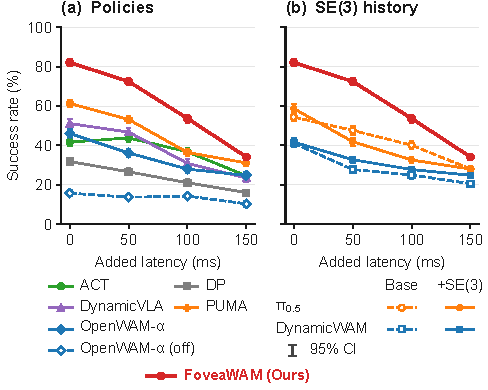
\includegraphics[width=\columnwidth]{latency/latency.pdf}
\caption{\textbf{Latency on \bench.} (a, b) SR versus added delay, for all policies (a) and for base versus +SE(3) variants (b), with 95\% CIs. (c) Paused
and native SR, colored by class as in Fig.~\ref{fig:teaser}, with rank changes
({\color{rankup}$\blacktriangle$}/{\color{rankdown}$\blacktriangledown$}).}
\label{fig:latency}
\end{figure}


\subsection{Dynamic Manipulation Results}
\label{sec:main_results}

\paragraph{Results on \bench.}
As shown in Table~\ref{tab:main}, \ours achieves the highest SR in all three settings.
At native latency, it reaches 82.1\%, \nativeLead{} points above the strongest baseline, PUMA
(61.4\%), and it has the highest or tied-highest SR on 13 of the 14 tasks, as
reported in the supplementary material. The margins are largest where a moving receptacle
or the target's orientation decides success. They reach 30 and 55 points on placement
into translating and rotating receptacles and 28 points on full wire passage. This
lead comes from the role-aware design. Given the same SE(3) history as input,
$\pi_{0.5}$ and DynamicWAM reach 58.7\% and 41.7\%, which is 23.4 and 40.4 points below
\ours.

\paragraph{Representation and latency.}
\ours leads both in how it represents the target's motion and in how quickly it acts.
With the world paused, inference costs no time, and \ours
still leads $\pi_{0.5}$+SE(3), which reads the same target poses, by 14.3 points. This
gap reflects the representation alone. At native latency, \ours loses 8.1 points and
$\pi_{0.5}$+SE(3) loses 17.3, so the gap widens to 23.4 points. Low latency alone is not
enough. ACT is the only method faster than \ours, but it reaches 41.6\%, which is 40.5
points below \ours. \ours leads at every added delay (Fig.~\ref{fig:latency}a). With 150\,ms
added, each chunk must cover a longer open-loop interval. Every method falls to
35\% or below, and the margin over PUMA narrows to 3.0 points.

% Table 2 is input here so that it floats next to the DOMINO results.
% Transcribed from results/domino_baselines/w5-formal-20261111.json (baselines) and results/domino_baselines/foveawam-epoch24-scenes.csv (FoveaWAM, step 2520).
\begin{table}[t]
\centering\footnotesize
\caption{\tablelang{\textbf{Quantitative comparison on DOMINO} \cite{domino}. SR (\%) on its 24 single-arm tasks, 8 Intercept and 16 Track. MS: manipulation score. Best and second best are highlighted.}{\textbf{DOMINO \cite{domino} 上的定量比较。}其 24 个单臂任务（8 个拦截、16 个跟踪）上的 SR（\%）。MS：操作得分。最佳与次佳已标出。}}
\label{tab:external}
\setlength{\tabcolsep}{2.2pt}
% Keep right padding so the MS highlight ends at the rule.
\begin{tabularx}{\linewidth}{@{}l*{4}{Y}}
\toprule
\tablelang{Method}{方法} & \tablelang{Intercept}{拦截} & \tablelang{Track}{跟踪} & \tablelang{All}{全部} $\uparrow$ & MS $\uparrow$ \\
\midrule
$\pi_{0.5}$ & 23.8 & 8.1 & 13.3 & 27.8 \\
DynamicWAM & 16.8 & \secondcell{31.9} & \secondcell{26.9} & \secondcell{41.4} \\
PUMA & \bestcell{36.3} & 12.2 & 20.2 & 35.4 \\
\oursentry & \secondcell{29.4} & \bestcell{55.5} & \bestcell{46.8} & \bestcell{62.0} \\
\bottomrule
\end{tabularx}
\end{table}


\paragraph{Motion input under latency.}
Precise motion input helps only when the action arrives in time
(Fig.~\ref{fig:latency}b). The SE(3) history raises $\pi_{0.5}$ by 9.4 points with the
world paused but by only 4.3 points at native latency. With 50 and 100\,ms added, it
lowers the SR of $\pi_{0.5}$ by 5.7 and 7.5 points, and the 95\% intervals do not
overlap. The history describes the target at capture time, so its value decays as the
action is delayed. \ours is designed to keep this value. It encodes the history
in 16 tokens and acts within one control period, so the history is still current when
the action executes. The history therefore adds 19.6 points to \ours at native latency,
against 4.3 points for $\pi_{0.5}$ (Table~\ref{tab:analysis}).

\paragraph{Paused evaluation.}
Pausing the world hides the cost of latency and reorders 9 of the 11 methods
(Fig.~\ref{fig:latency}c). The two OpenWAM-$\alpha$ deployments share one policy and
reach 58.7\% and 58.4\% with the world paused. At native latency, with p95 of 151.7 and
466.3\,ms, they reach 46.1\% and 15.8\%. The three slowest methods all lose
rank, and the strongest baseline changes from $\pi_{0.5}$+SE(3) to PUMA.

\paragraph{Results on DOMINO.}
DOMINO \cite{domino} has its own tasks, demonstrations, and evaluator. We train \ours,
$\pi_{0.5}$, DynamicWAM, and PUMA on its 24 single-arm Franka tasks. \ours achieves
46.8\% SR and 62.0 MS, 19.9 and 20.6 points above the strongest baseline, DynamicWAM
(Table~\ref{tab:external}). The evaluator pauses physics during inference, so latency
brings no advantage. This lead therefore shows the value of the role-aware
representation itself. With its lead in the paused setting of \bench, \ours leads
whether or not latency is counted. The margin is largest on the 16
Track tasks, where the robot must keep a consistent pose relative to the moving target.
The SE(3) trajectory describes the target's future poses directly, and \ours reaches
55.5\% against 31.9\%. PUMA leads on the 8 Intercept tasks, which require a
single contact with the target (36.3\% against 29.4\%).

\subsection{Ablation Study}
\label{sec:principles}
Table~\ref{tab:analysis} ablates each part of the role-aware design. All
variants except \emph{w/o history} change only the training supervision and run at the
latency of \ours.

% Table 3 is input after the section start so that it floats to the top of the next column.
% Transcribed from se3-wam-focused/research/evidence/hard/ablation-bf16/checkpoint-matrix64.json (latest.pt for each model).
% Rot./Ctx. are task-balanced means over the groups of Table tab:roles, native latency.
% The Paused column is reported in supp_analysis.tex (Table tab:supp_analysis).
% D4RT (CVPR 2026, Table 9) shading. With r = |Delta| / max(|Delta|) within each column,
% mix white with 50*sqrt(r)% red for drops or 50*r% green for gains.
\begin{table}[t]
\centering\footnotesize
\caption{\tablelang{\textbf{Ablation results on \bench.} SR (\%) of \ours and its change for each variant ($\Delta$, points; red: drop, green: gain). Rot./Ctx.: rotation-sensitive and context-active tasks.}{\textbf{\bench 上的消融结果。}\ours 的 SR（\%）及各变体的变化（$\Delta$，百分点；红色为下降，绿色为提升）。Rot./Ctx.：旋转敏感组与环境活跃组。}}
\label{tab:analysis}
\setlength{\tabcolsep}{2.2pt}
% Equal-width numeric columns retain padding at the right edge for the cell colors.
\begin{tabularx}{\linewidth}{@{}l*{4}{Y}}
\toprule
 & \multicolumn{2}{c}{\tablelang{Success rate, all tasks}{SR，全部任务}} & \multicolumn{2}{c}{\tablelang{Groups (Native)}{任务组（原生）}}\\
\cmidrule(lr){2-3}\cmidrule(l){4-5}
 & \tablelang{Native}{原生} & +150\,ms & Rot. & Ctx.\\
\midrule
\textbf{\ours} & \textbf{82.1} & \textbf{34.1} & \textbf{80.4} & \textbf{82.7}\\
\midrule
\multicolumn{5}{@{}l}{\textit{\tablelang{Precision allocation}{精度分配}}}\\
\quad \tablelang{Uniform coarse flow}{统一粗粒度流} & \cellcolor{red!24.0}$-$4.5 & \cellcolor{red!19.2}$-$0.5 & \cellcolor{red!29.9}$-$8.6 & \cellcolor{red!50.0}$-$4.6\\
\quad \tablelang{Uniform fine flow}{统一精细流} & \cellcolor{green!2.0}+0.8 & \cellcolor{red!25.7}$-$0.9 & \cellcolor{red!18.8}$-$3.4 & \cellcolor{red!37.6}$-$2.6\\
\quad \tablelang{w/o flow}{无场景流} & \cellcolor{red!23.1}$-$4.2 & \cellcolor{red!32.1}$-$1.4 & \cellcolor{red!34.9}$-$11.7 & \cellcolor{red!46.0}$-$3.9\\
\multicolumn{5}{@{}l}{\textit{\tablelang{Target motion history}{目标运动历史}}}\\
\quad \tablelang{w/o history}{无目标历史} & \cellcolor{red!50.0}$-$19.6 & \cellcolor{green!2.9}+0.2 & \cellcolor{red!50.0}$-$24.0 & \cellcolor{red!35.4}$-$2.3\\
\multicolumn{5}{@{}l}{\textit{\tablelang{Future supervision}{未来监督}}}\\
\quad \tablelang{w/o future}{无未来监督} & \cellcolor{red!23.4}$-$4.3 & \cellcolor{red!50.0}$-$3.4 & \cellcolor{red!36.2}$-$12.6 & \cellcolor{red!33.8}$-$2.1\\
\quad \tablelang{w/o $\mathcal{L}_{\text{aux}}$}{无 $\mathcal{L}_{\text{aux}}$} & \cellcolor{red!18.2}$-$2.6 & \cellcolor{red!37.4}$-$1.9 & \cellcolor{red!34.8}$-$11.6 & \cellcolor{green!1.1}+0.1\\
\bottomrule
\end{tabularx}
\end{table}


\paragraph{Effect of target motion history.}
The pose history is the most important input. Removing it while keeping the
current pose reduces SR by 19.6 points at native latency and by 24.0 points on
rotation-sensitive tasks. The drop is the same with the world paused (19.5 points). A
single pose shows where the target is but not how it moves. The history supplies the
velocity and acceleration that commands must anticipate.

\paragraph{Effect of role-aware prediction.}
Each role needs its own form of prediction. Replacing the SE(3) trajectory with flow at
the density of the surroundings reduces SR by 4.5 points, and by 8.6 points on
rotation-sensitive tasks. At this density, the few patches on the target cannot
determine its rotation. A $16\times$ denser flow recovers the overall SR but still
trails \ours by 3.4 and 2.6 points on rotation-sensitive and context-active tasks.
Removing the sparse flow reduces SR by 4.2 points, and by 11.7 points on
rotation-sensitive tasks, because the flow shapes the patch tokens that the action
stream reads near contact. One target trajectory and 196 flow points thus match
3{,}136 uniform flow points overall and surpass them where rotation and context matter.

\paragraph{Effect of future supervision.}
Supervising only the current target state instead of its future reduces SR by 4.3
points, and by 12.6 points on rotation-sensitive tasks, although the prediction heads
never run at deployment. Prediction thus helps through the representation it
shapes. The appearance losses $\mathcal L_{\rm aux}$ also help,
mainly on rotation-sensitive tasks.

\paragraph{Prediction in a moving world.}
The three variants that weaken future prediction (\emph{uniform coarse flow},
\emph{w/o flow}, \emph{w/o future}) each lose more than 4 points at native latency
but none with the world paused. With the world paused, a policy replans every 50\,ms
and executes only the command for the capture time. At native latency, the
15.1\,ms inference of \ours delays execution to the next control boundary, 50\,ms after
capture. The representation must then encode where the target will be. Removing the history or
$\mathcal L_{\rm aux}$ instead lowers SR in both settings. Paused evaluation hides the
value of prediction, and \bench reveals it.

\subsection{Real-Robot Evaluation}
\label{sec:real}

\begin{figure*}[t]
\centering
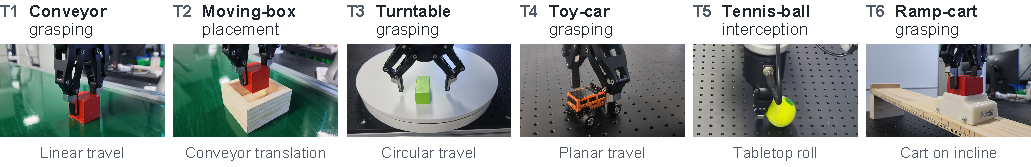
\includegraphics[width=\textwidth]{Fig6/outputs/polished/fig6.pdf}
\caption{\textbf{Real-robot task setups.}
The tasks include grasping a block from a conveyor belt, placing a block in a moving box,
grasping a block from a turntable, grasping a moving toy car, intercepting a rolling tennis ball,
and grasping a block from a ramp cart.
The tennis ball panel shows a frame from the demonstration video.}
\label{fig:real_trials}
\end{figure*}


We evaluate on six dynamic tasks with \cfgRobot{} (Fig.~\ref{fig:real_trials}). All methods are trained on the same 600 teleoperated
demonstrations and evaluated for 20 trials per task. \ours starts from a
DROID-pretrained base \cite{droid} and uses RGB-D and online target pose estimates from
one fixed camera. ACT and $\pi_{0.5}$ use RGB images from the fixed and wrist cameras. Further
details on the tasks and platform are in the supplementary material.

% Transcribed from the author-provided six-task real-robot results. All pools 120 trials per method.
\begin{table}[t]
\centering\footnotesize
\caption{\tablelang{\textbf{Real-robot results.} SR (\%) over 20 trials per task.}{\textbf{真机结果。}每项任务试验 20 次，报告成功率（\%）。}}
\label{tab:real}
\setlength{\tabcolsep}{1.2pt}
\begin{tabular}{@{}l*{7}{c}}
\toprule
\tablelang{Method}{方法}
& \makecell{\tablelang{Conveyor}{传送带}\\\tablelang{grasp}{抓取}}
& \makecell{\tablelang{Box}{移动盒}\\\tablelang{place}{放置}}
& \makecell{\tablelang{Turntable}{转盘}\\\tablelang{grasp}{抓取}}
& \makecell{\tablelang{Toy car}{玩具车}\\\tablelang{grasp}{抓取}}
& \makecell{\tablelang{Ball}{网球}\\\tablelang{intercept}{拦截}}
& \makecell{\tablelang{Ramp cart}{斜坡小车}\\\tablelang{grasp}{抓取}}
& \tablelang{All}{总体} $\uparrow$ \\
\midrule
ACT & 0 & 0 & 0 & 0 & 10 & 0 & 1.7 \\
$\pi_{0.5}$ & 45 & 75 & 30 & 20 & 15 & 0 & 30.8 \\
\makecell[l]{\oursname\\\tablelang{(Ours)}{（本文）}} & \bestcell{70} & \bestcell{80} & \bestcell{60} & \bestcell{35} & \bestcell{35} & \bestcell{10} & \bestcell{48.3} \\
\bottomrule
\end{tabular}
\end{table}


On the robot, the scene keeps moving during inference, as in \emph{Native}. \ours
achieves the highest SR on all six tasks and 48.3\% overall, 17.5 points above
$\pi_{0.5}$ (Table~\ref{tab:real}). The largest gains, 30 and 25 points, are on
turntable and conveyor grasping. ACT, the fastest policy, succeeds in only 2 of 120
trials. On ramp cart grasping, the hardest task, only \ours succeeds
(2 of 20 trials).
